\section{Название приложения}
\label{sec:Appendix_}

\begin{figure*}[!h]
	\centering
	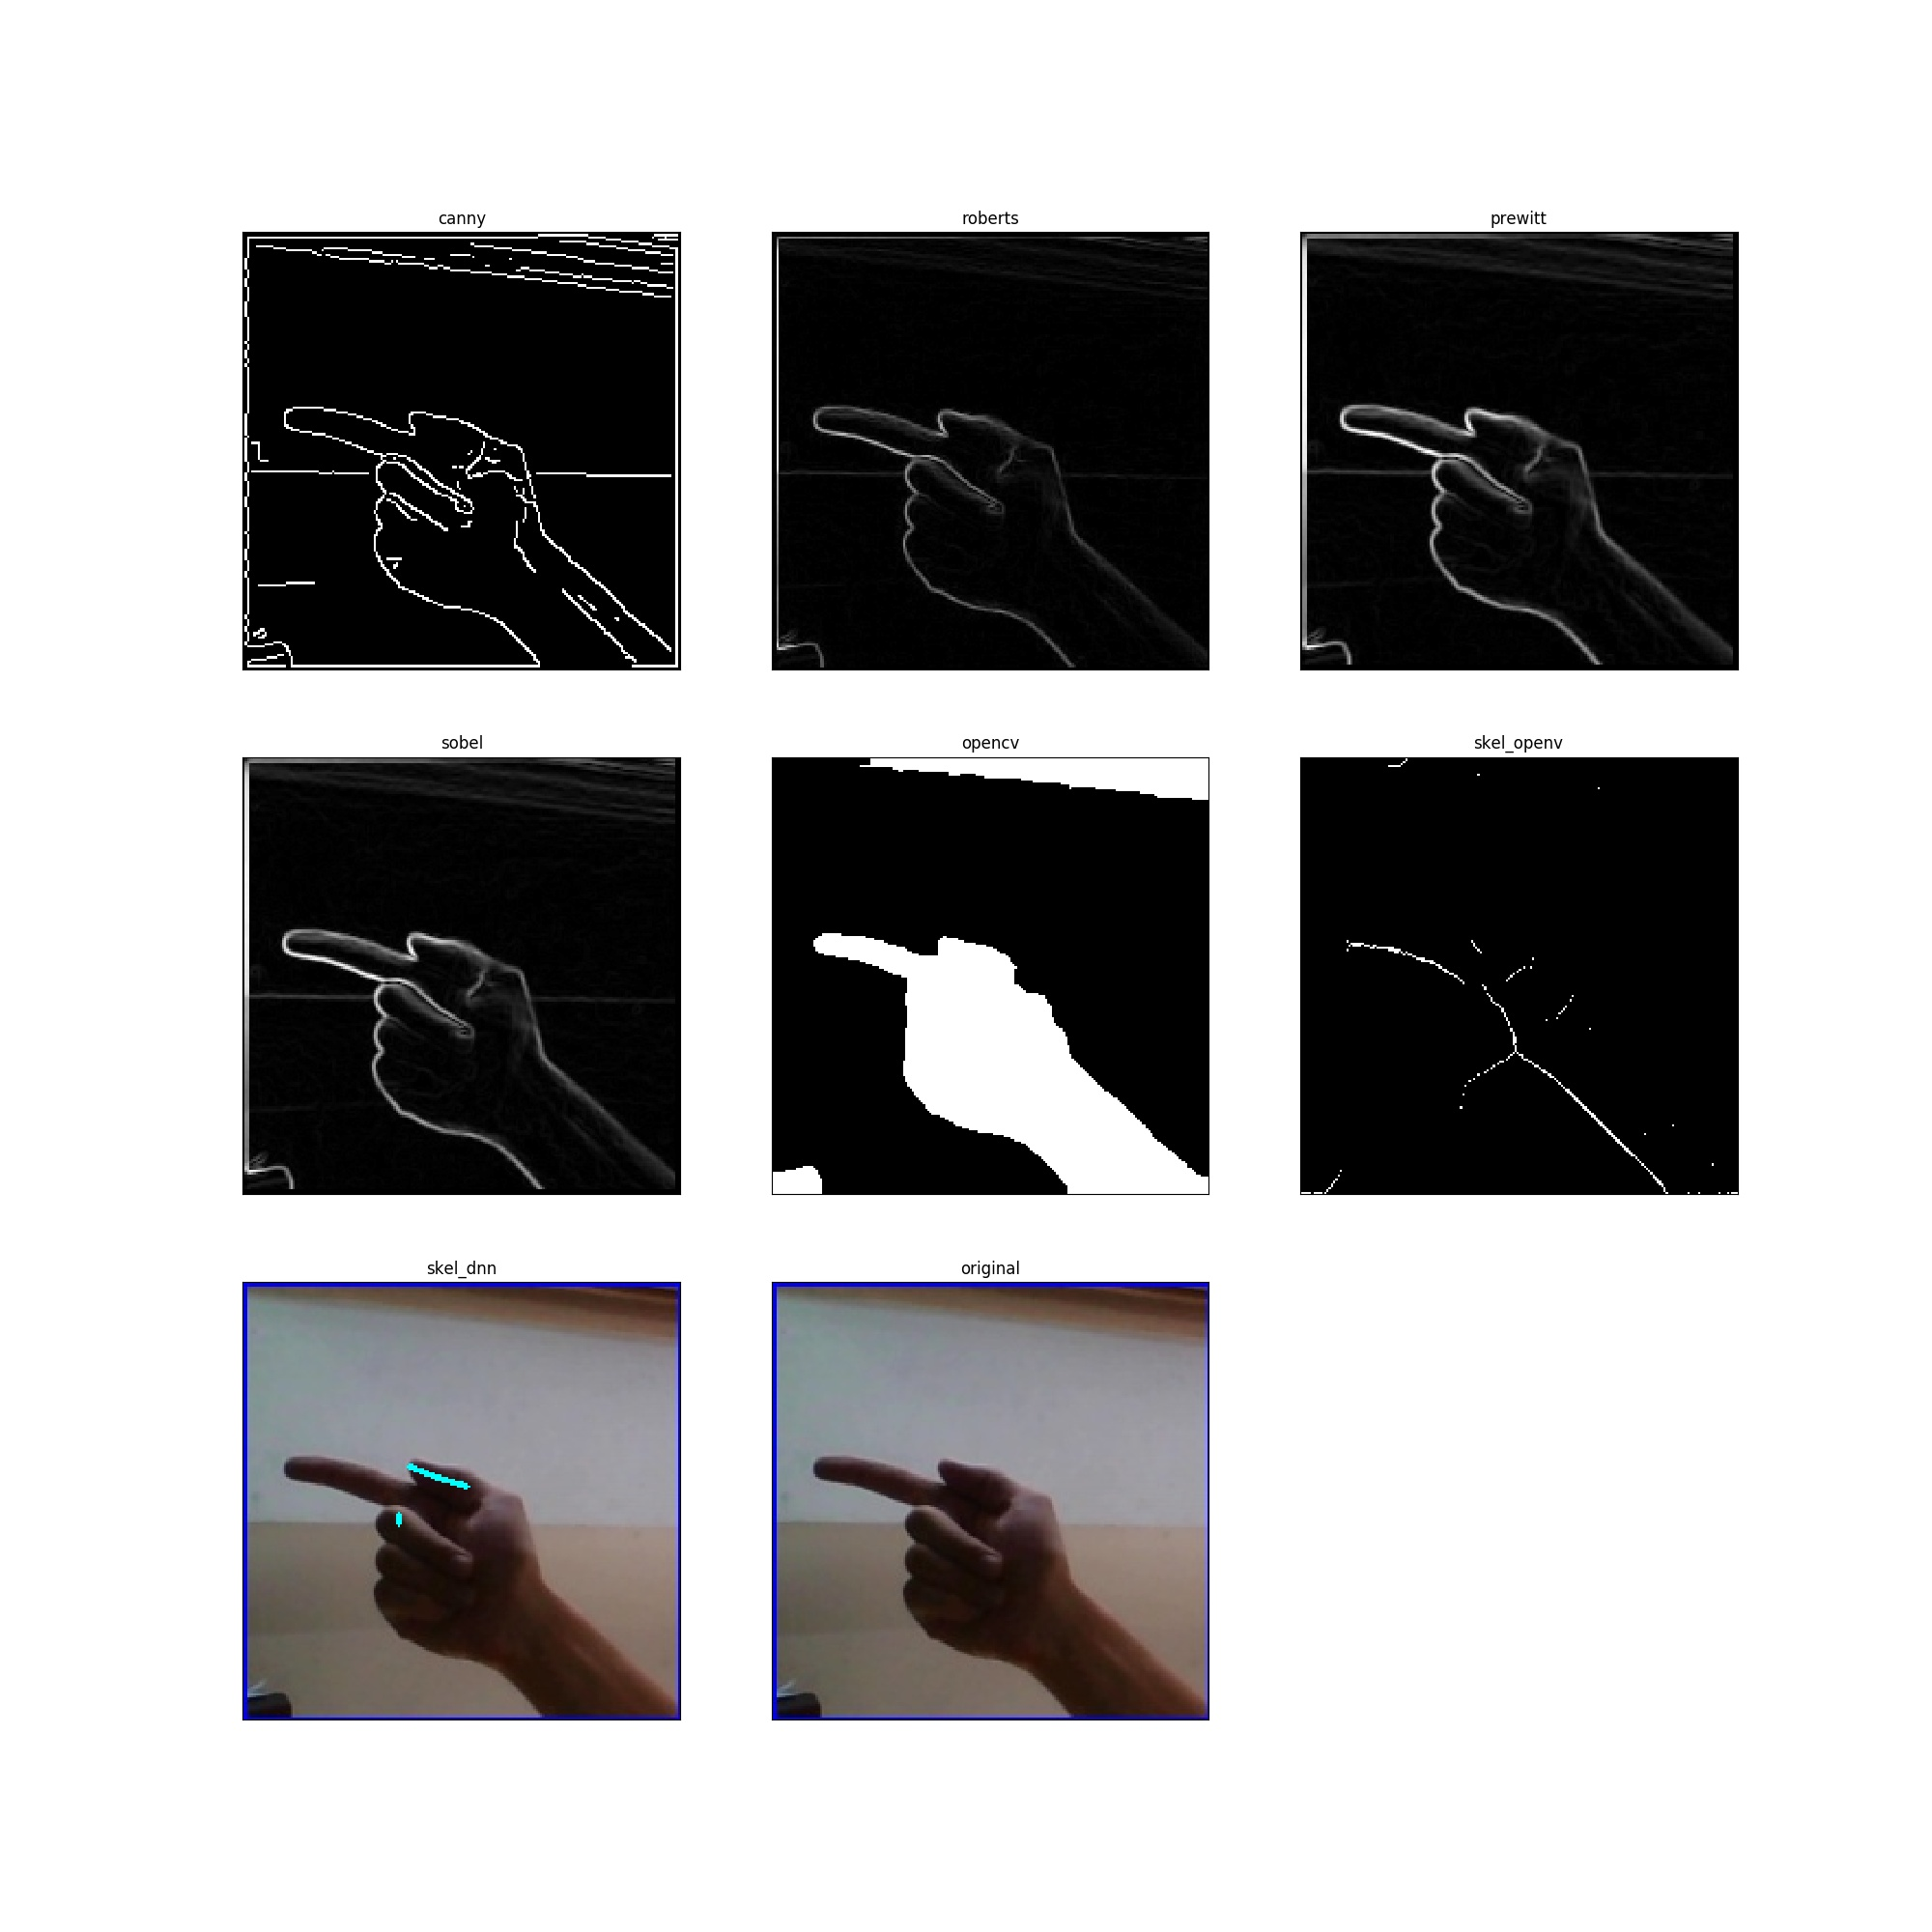
\includegraphics[width=\textwidth,keepaspectratio]{figures/ru/asl.jpg}
	\caption{Результат работы алгоритмов (в секундах) на наборе данных ASL Alphabet}
	\label{fig:asl}
\end{figure*}

\begin{figure*}[!h]
	\centering
	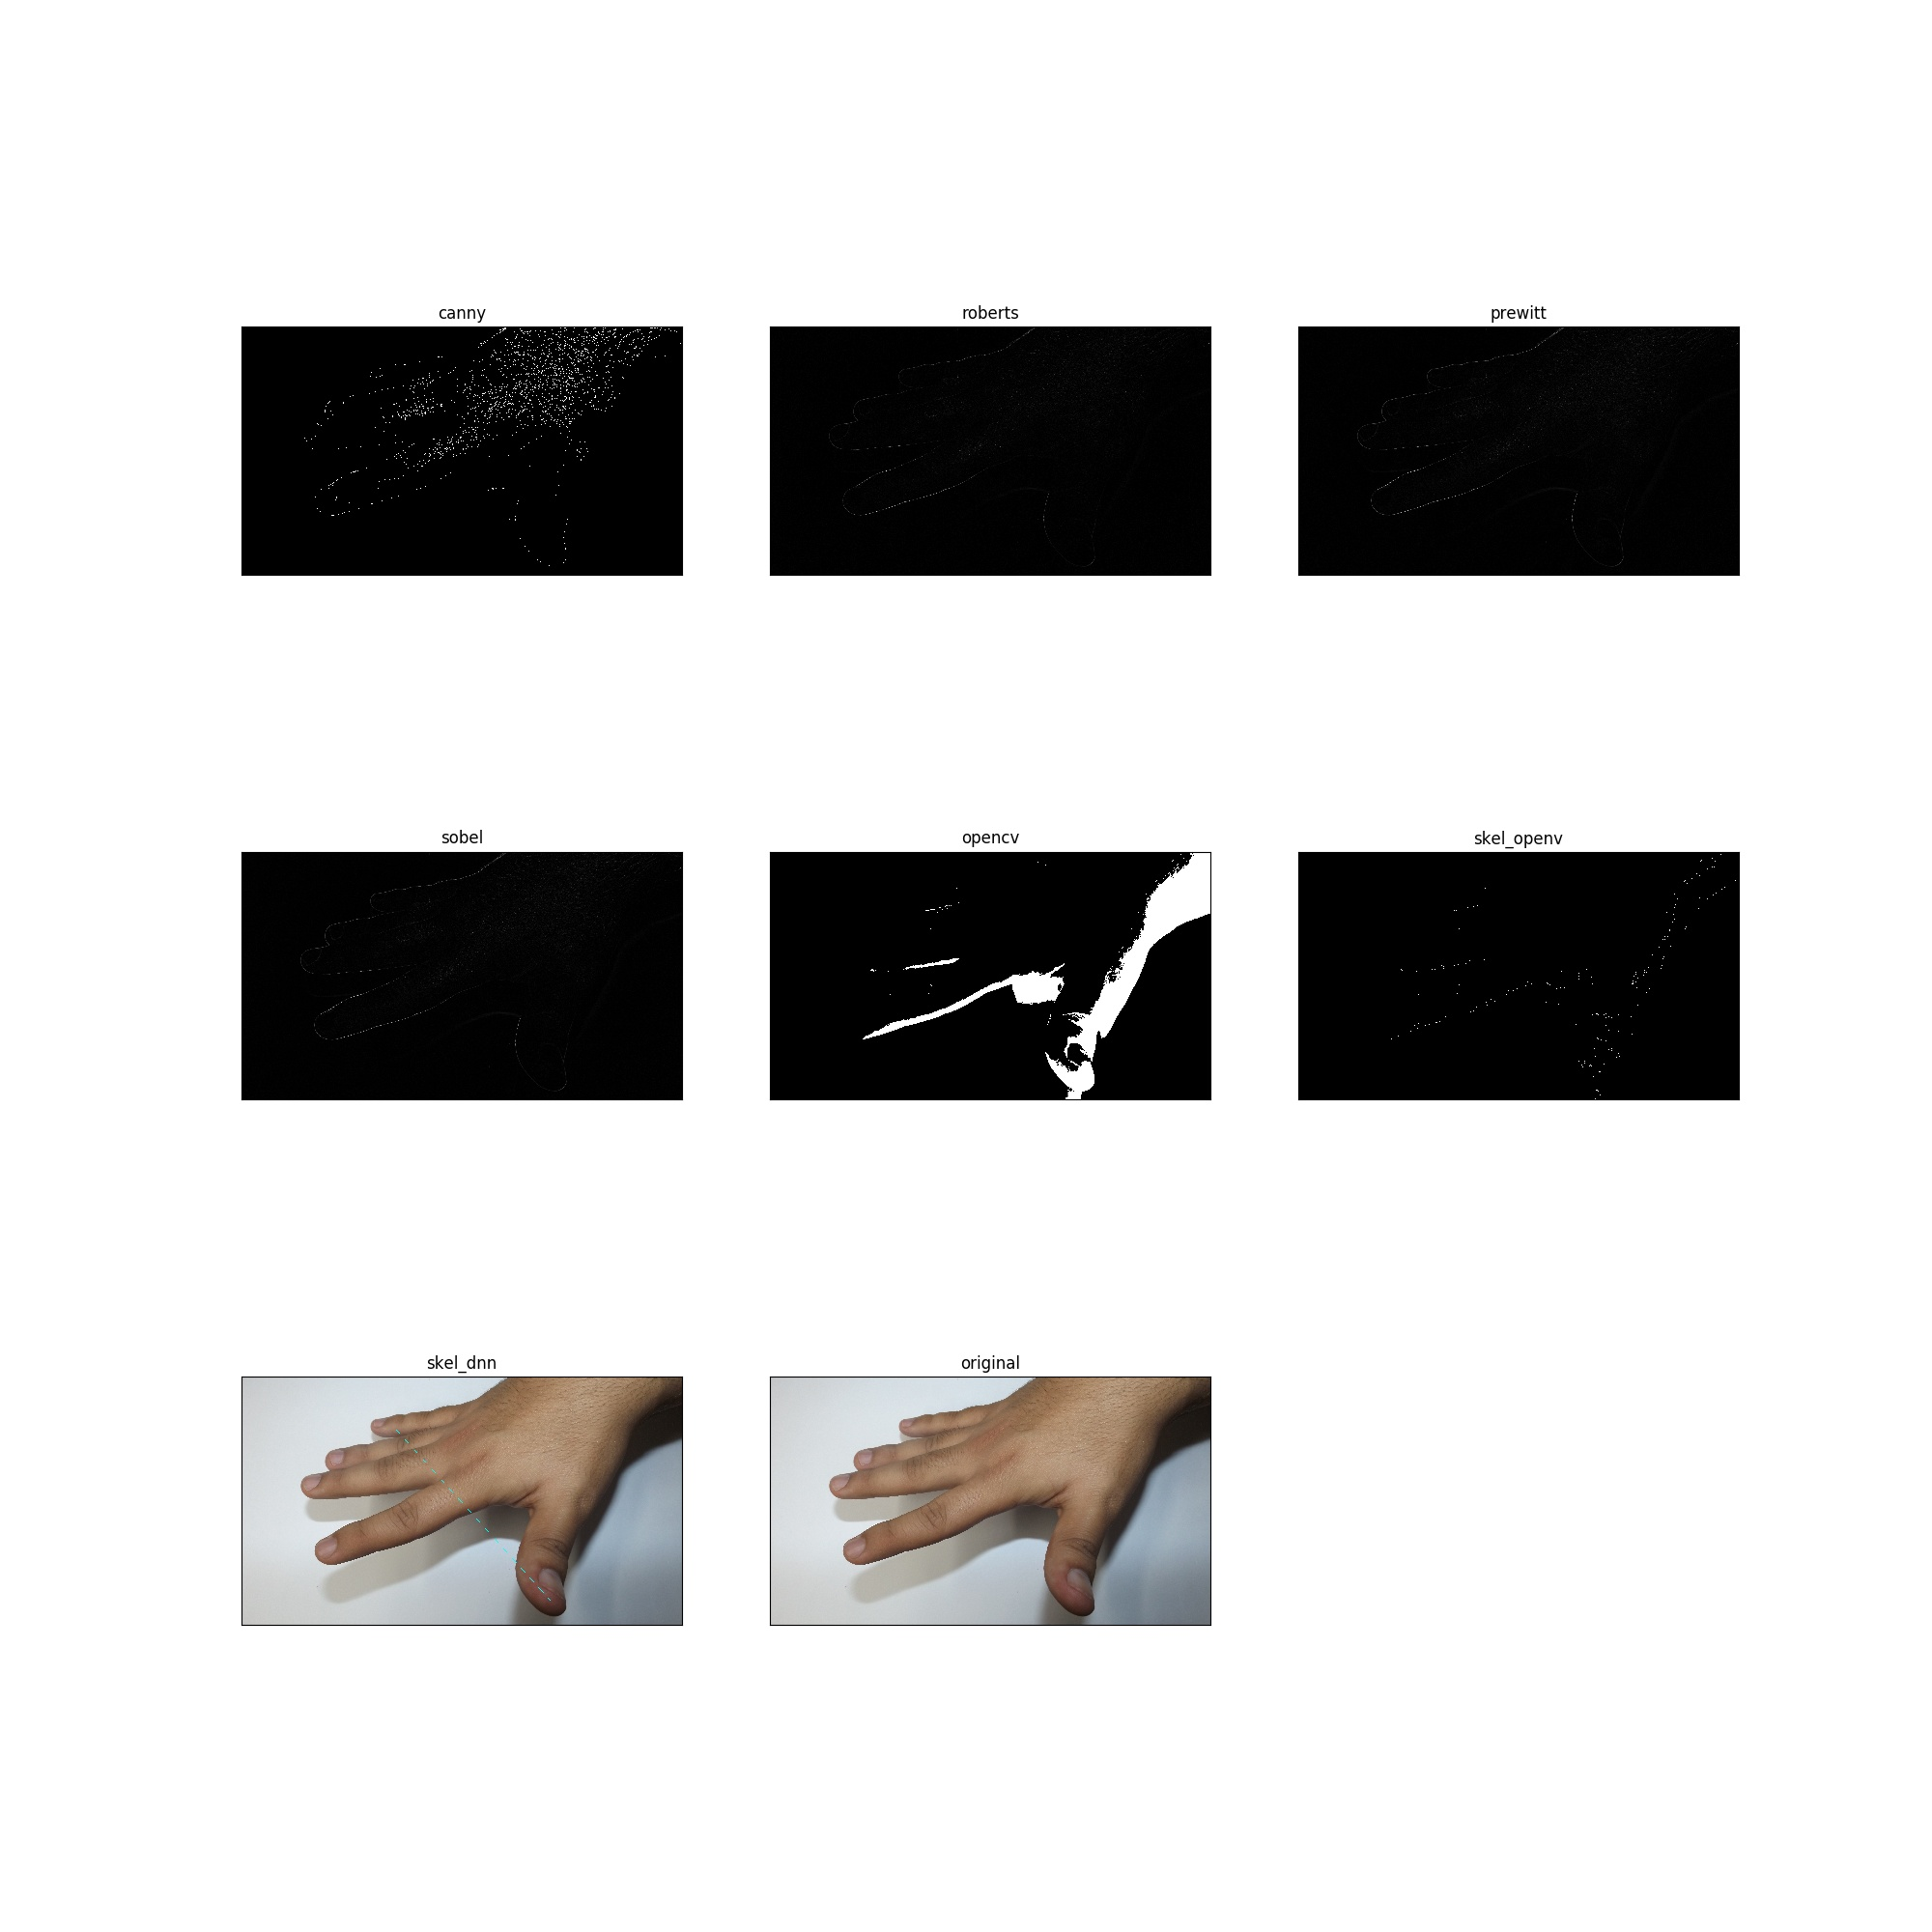
\includegraphics[width=\textwidth,keepaspectratio]{figures/ru/coombian.jpg}
	\caption{Результат работы алгоритмов (в секундах) на наборе данных Hand Gesture of the Colombian sign language}
	\label{fig:colombian}
\end{figure*}

\begin{figure*}[!h]
	\centering
	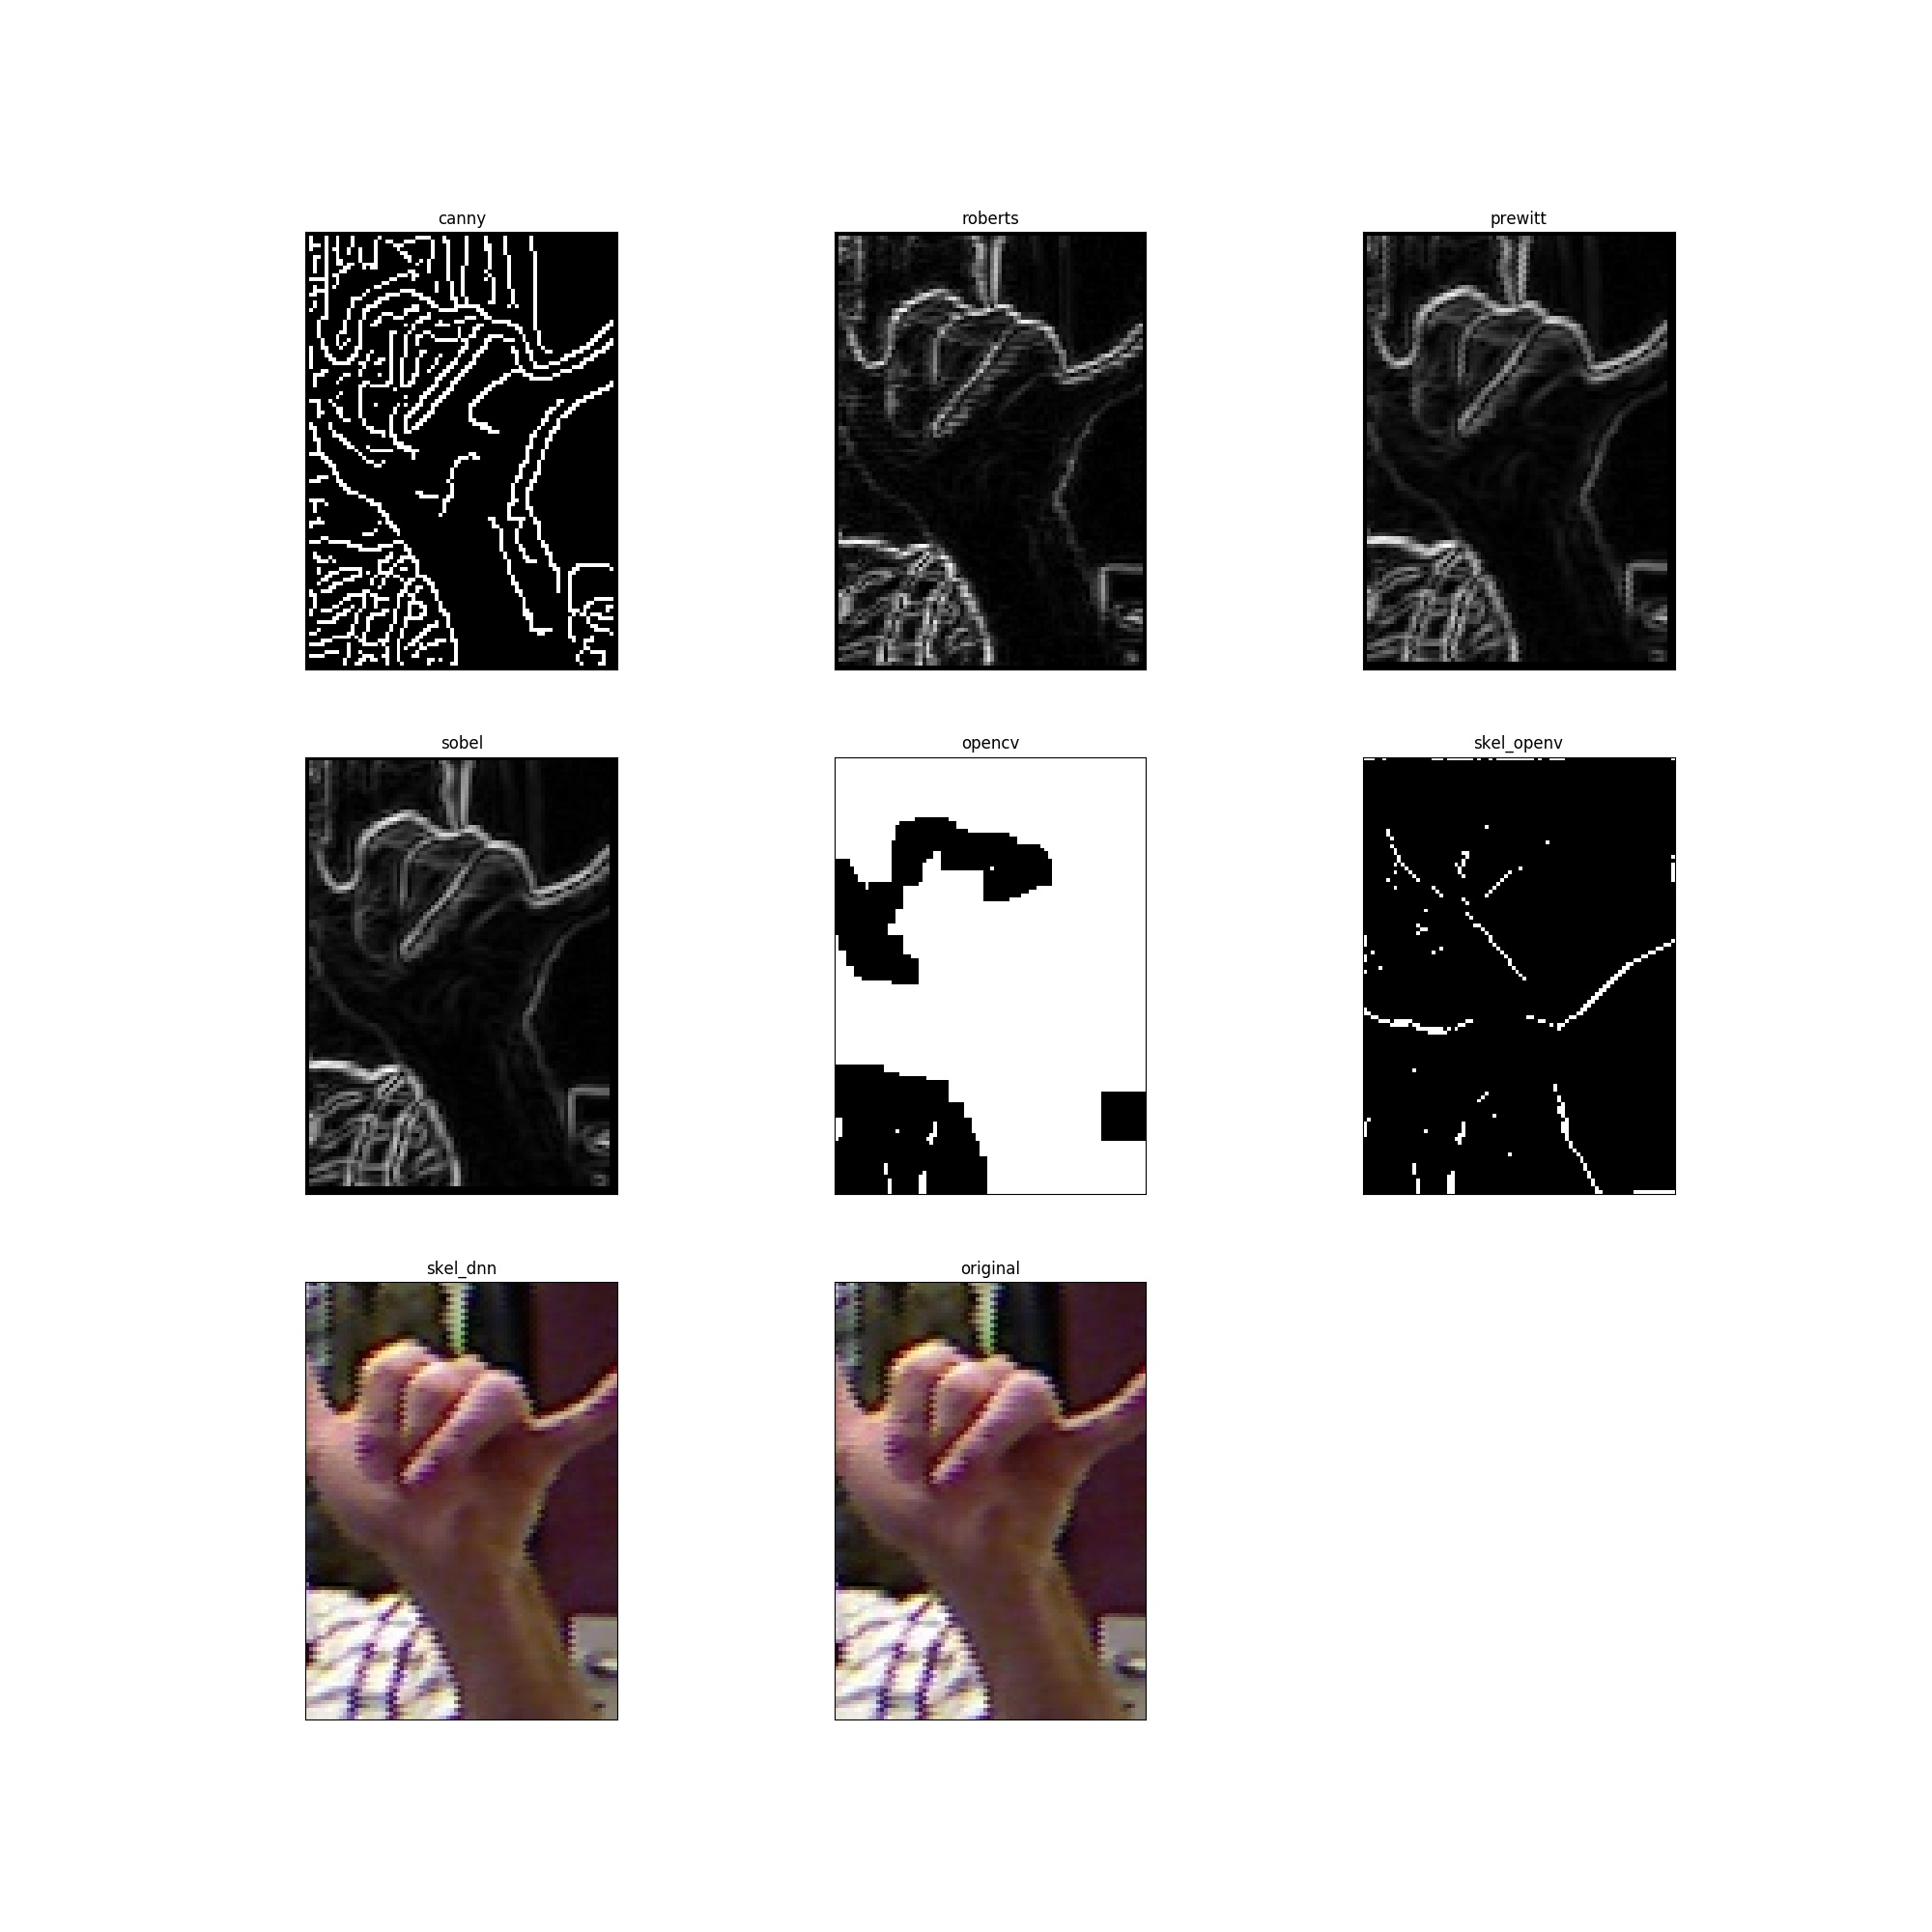
\includegraphics[width=\textwidth,keepaspectratio]{figures/ru/asl2.jpg}
	\caption{Результат работы алгоритмов (в секундах) на наборе данных ASL Fingerspelling Images}
	\label{fig:asl2}
\end{figure*}

\begin{figure*}[!h]
	\centering
	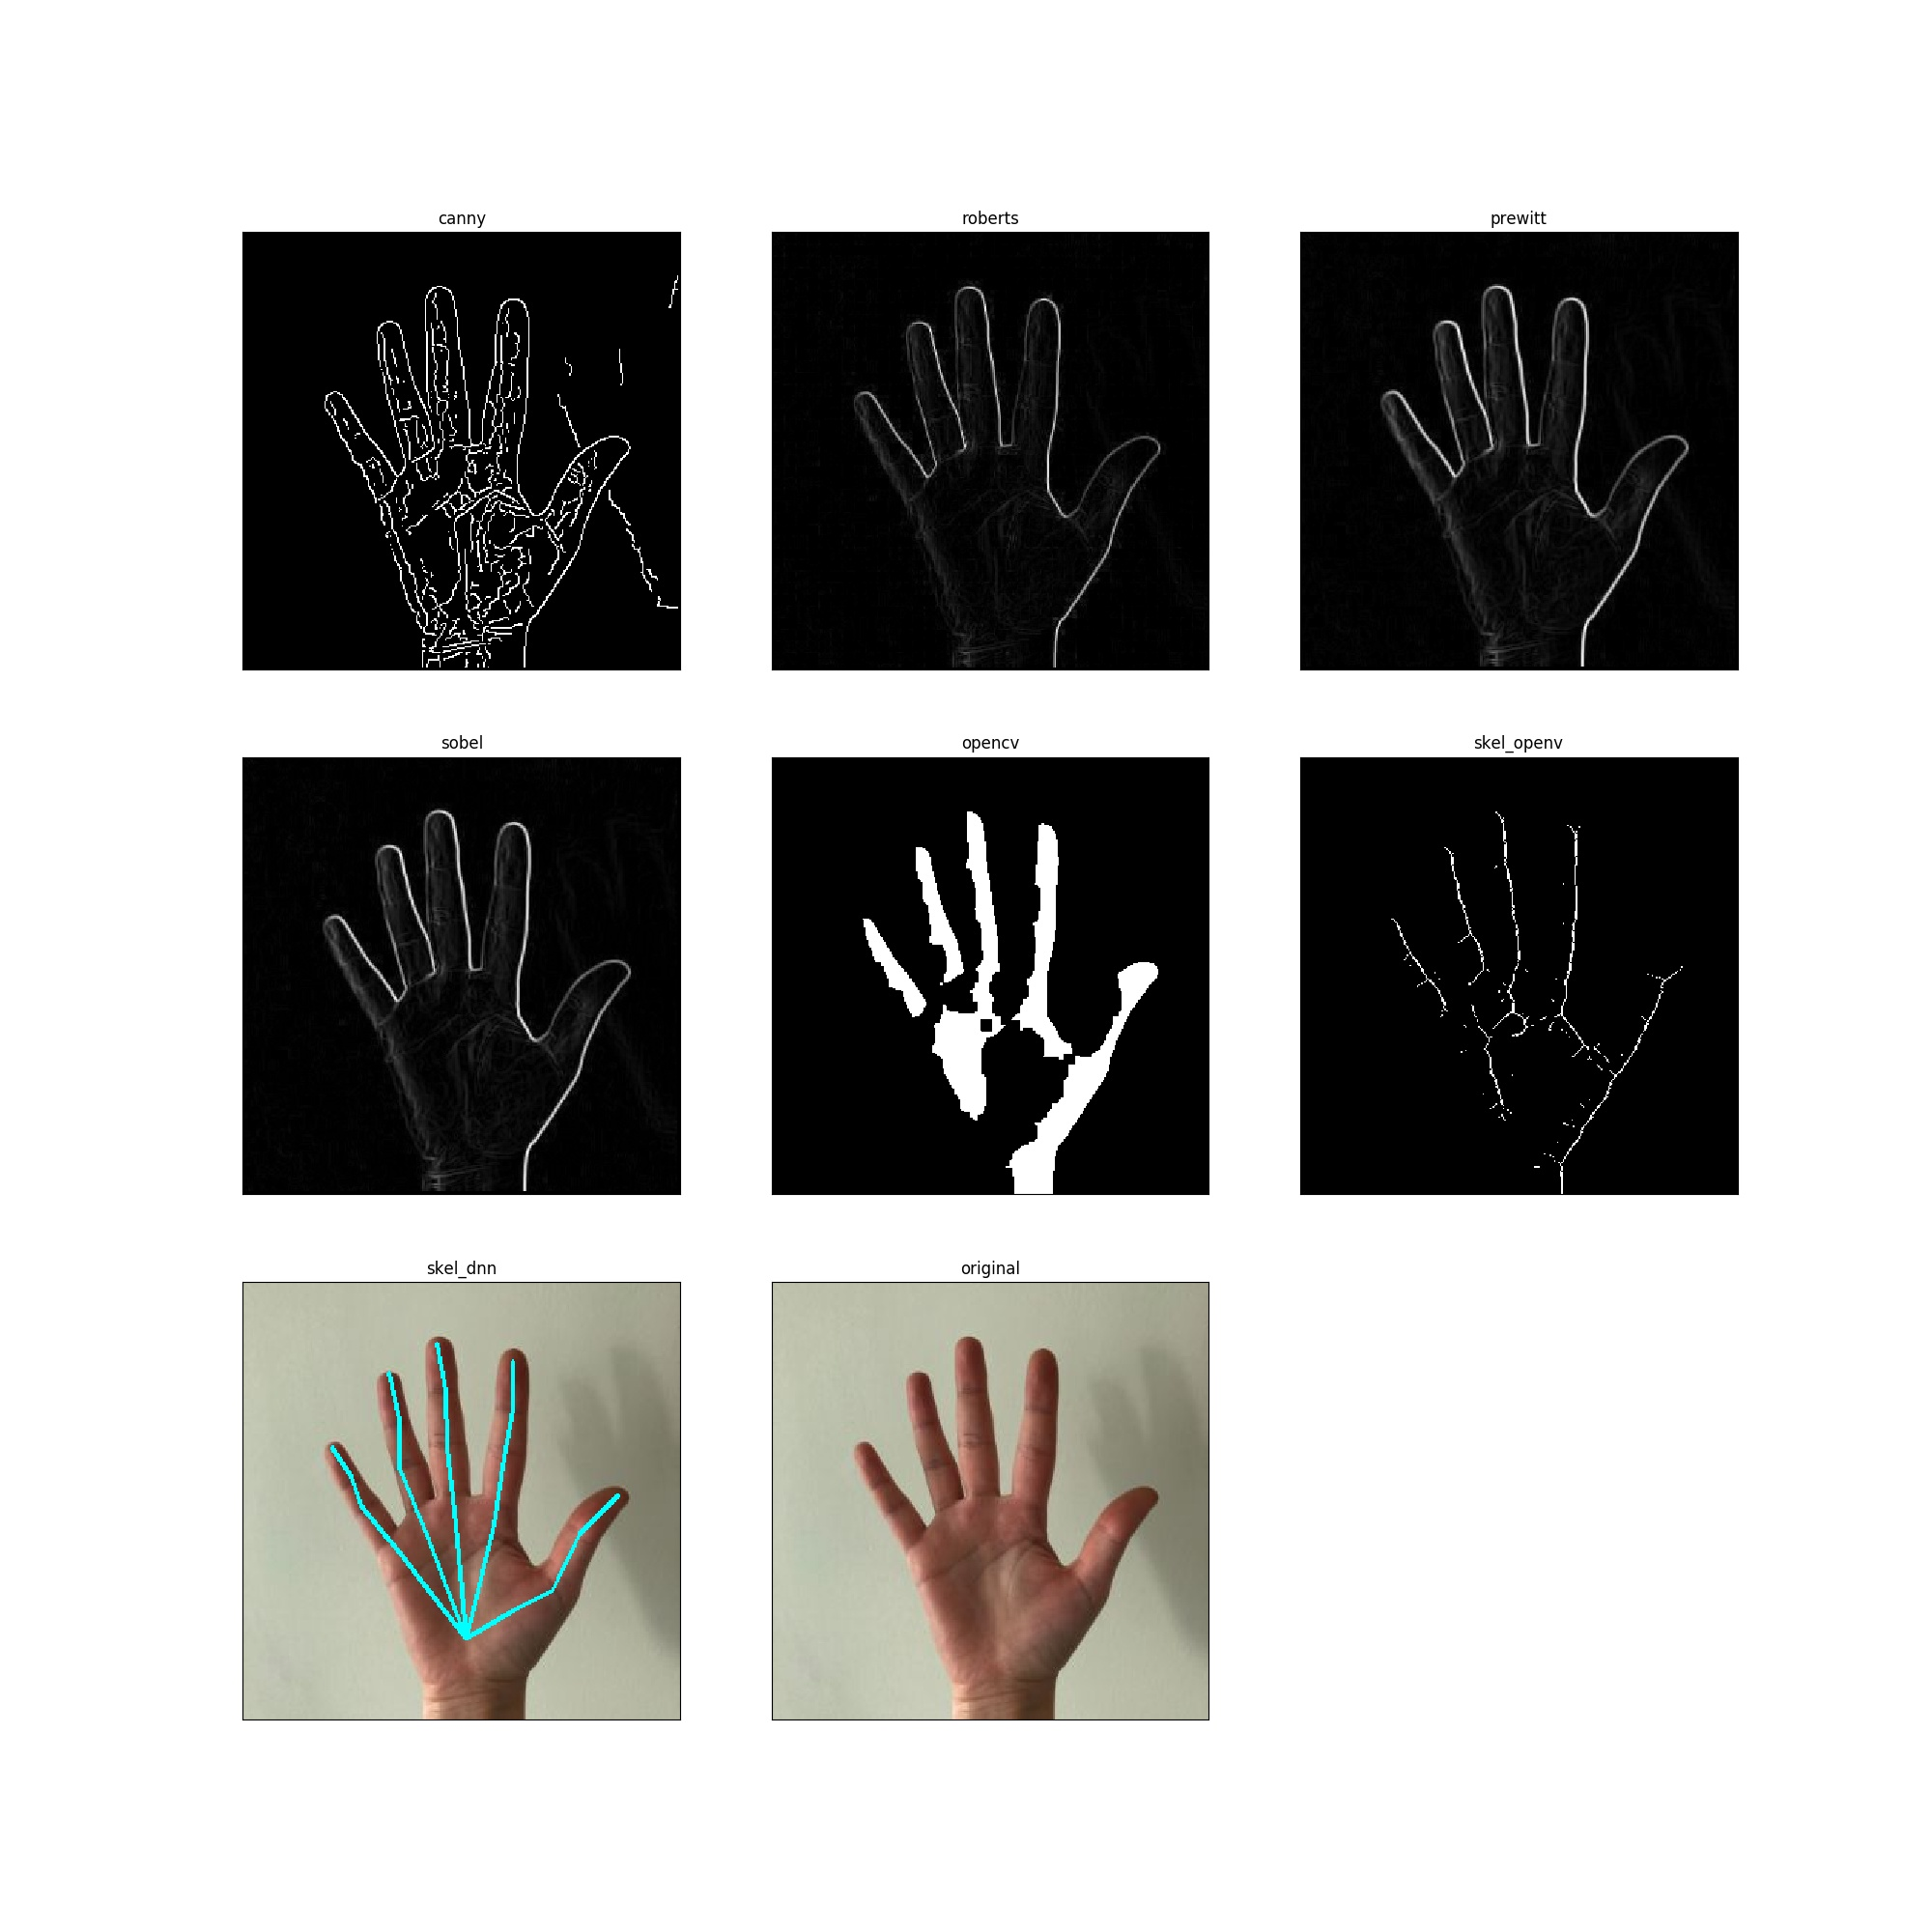
\includegraphics[width=\textwidth,keepaspectratio]{figures/ru/datamix.jpg}
	\caption{Результат работы алгоритмов (в секундах) на наборе данных sign language between 0 9}
	\label{fig:datamix}
\end{figure*}

\begin{table*}[!h]
\caption{Время работы алгоритмов (в секундах) на наборе данных ASL Alphabet}
\label{tab:asl-alphaber}
\setlength{\arrayrulewidth}{1.05 pt}
\renewcommand{\arraystretch}{1.1}
\begin{tabular*}{1.0\textwidth}{@{\extracolsep{\fill}}|c|c|c|c|}
	\hline
	Название алгоритма & Минимальное время & Максимальное время & Среднее время \\
	\hline
	Оператор Кэнни & 0.1783 & 0.4642 & 0.2553 \\
	Оператор Робертса & 0.0687 & 0.1252 & 0.0852 \\
	Оператор Прюитт & 0.1175 & 0.2211 & 0.1424  \\
	Оператор Собеля & 0.1177 & 0.3112 & 0.1527 \\
	Выделение силуэта & 0.0668 & 0.2101 & 0.0901 \\
	\specialcell{Морфологическое \\ построение скелета} & 0.2084 & 1.2112 & 0.3068 \\
	\specialcell{Построение скелета \\ по ключевым точкам} & 1.408 & 3.4571 & 2.042 \\
	\hline
\end{tabular*}
\end{table*}

\begin{table*}[!h]
\caption{Время работы алгоритмов (в секундах) на наборе данных Hand Gesture of the Colombian sign language}
\label{tab:colombian-alphaber}
\setlength{\arrayrulewidth}{1.05 pt}
\renewcommand{\arraystretch}{1.1}
\begin{tabular*}{1.0\textwidth}{@{\extracolsep{\fill}}|c|c|c|c|}
	\hline
	Название алгоритма & Минимальное время & Максимальное время & Среднее время \\
	\hline
	Оператор Кэнни & 53.5126 & 72.6076 & 62.971 \\
	Оператор Робертса & 22.2837 & 54.2706 & 25.8842 \\
	Оператор Прюитт & 38.7491 & 99.2961 & 46.5944 \\
	Оператор Собеля & 38.8739 & 104.1867 & 46.9016 \\
	Выделение силуэта & 22.3001 & 32.8930 & 23.5992 \\
	\specialcell{Морфологическое \\ построение скелета} & 65.3335 & 88.3565 & 69.0014 \\
	\specialcell{Построение скелета \\ по ключевым точкам} & 3.0844 & 4.2156 & 3.2775 \\
	\hline
\end{tabular*}
\end{table*}

\begin{table*}[!h]
\caption{Время работы алгоритмов (в секундах) на наборе данных ASL Fingerspelling Images}
\label{tab:asl2-alphaber}
\setlength{\arrayrulewidth}{1.05 pt}
\renewcommand{\arraystretch}{1.1}
\begin{tabular*}{1.0\textwidth}{@{\extracolsep{\fill}}|c|c|c|c|}
	\hline
	Название алгоритма & Минимальное время & Максимальное время & Среднее время \\
	\hline
	Оператор Кэнни & 0.0193 & 0.0816 & 0.0545 \\
	Оператор Робертса & 0.0111 & 0.0476 & 0.0286 \\
	Оператор Прюитт & 0.0179 & 0.0864 & 0.0495 \\
	Оператор Собеля & 0.0217 & 0.0847 & 0.0469 \\
	Выделение силуэта & 0.0114 & 0.0506 & 0.0277 \\
	\specialcell{Морфологическое \\ построение скелета} & 0.0343 & 0.1852 & 0.0884 \\
	\specialcell{Построение скелета \\ по ключевым точкам} & 0.6251 & 3.3092 & 1.5665 \\
	\hline
\end{tabular*}
\end{table*}

\begin{table*}[!h]
	\caption{Время работы алгоритмов (в секундах) на наборе данных sign language between 0 9}
	\label{tab:datamix-alphaber}
	\setlength{\arrayrulewidth}{1.05 pt}
	\renewcommand{\arraystretch}{1.1}
	\begin{tabular*}{1.0\textwidth}{@{\extracolsep{\fill}}|c|c|c|c|}
		\hline
		Название алгоритма & Минимальное время & Максимальное время & Среднее время \\
		\hline
		Оператор Кэнни & 0.333 & 0.7686 & 0.4708 \\
		Оператор Робертса & 0.1566 & 0.246 & 0.1778 \\
		Оператор Прюитт & 0.271 & 0.3751 & 0.3027 \\
		Оператор Собеля & 0.2718 & 0.655 & 0.3295 \\
		Выделение силуэта & 0.1486 & 0.4709 & 0.2085 \\
		\specialcell{Морфологическое \\ построение скелета} & 0.4471 & 1.637 & 0.6518 \\
		\specialcell{Построение скелета \\ по ключевым точкам} & 1.4346 & 3.2976 & 2.0723 \\
		\hline
	\end{tabular*}
\end{table*}